\chapter[Regularized Transport and Mapping Estimation]{\texorpdfstring{Regularized Transport and \\ Mapping Estimation}{Regularized Transport and Mapping Estimation}}\label{DualPlanEst}

In the following, $\Omega_1 \subseteq \R^{n_1}$, $\Omega_2 \subseteq \R^{n_2}$ and $\Omega_1 \times \Omega_2 =: \Omega \subseteq \R^{n_1 + n_2}$ will always be compact for some $\NinN[n_1, n_2]$.

We will first introduce regularized optimal transport. The process of regularization imposes an additional penalty on the objective function of an optimization problem. This can serve multiple purposes: regularizing an ill-posed problem can allow for an approximate solution, result in uniqueness of the solution or, especially in the case covered in this thesis, allow for duality results which net themselves for further applications.

The barycentric projection will then be used to obtain a transport map from the optimal regularized transport plan. Due to the explicit computation of these transport solutions often being impractical for applications, it is necessary to estimate optimal transport plans and maps. This is traditionally done by formulating a regulariyed dual problem and applying the Sinkhorn algorithm, however this particular algorithm is not suited to handle large-scale problems. Hence, a different approach involving neural networks and stochastic mapping estimation is required.

The first sections on regularization and the corresponding regularized dual problem follow\ \cite{Cla2021} closely, while the last section is adapted from\ \cite[Section~3 and Section~4]{Seg2018}.

\section{Regularized Optimal Transport}\label{RegOT}

There are multiple ways in which regularization can take place, however we will focus on \textit{entropic regularization}. This form of regularization deals with measurable functions with finite entropy, i.e.~for $f \in \MF{\Omega}{\R}$
\[ E(f) := \int\limits_\Omega \big\vert f(z) \big\vert \log\big( \vert f(z) \vert \big)~\D[z] < \infty, \]
where $0 \cdot \log(0) := 0$. From here we can define
\[ \LLL := \left\{ f \in \MF{\Omega}{\R} : \int\limits_\Omega \big\vert f(z) \big\vert \log^+\big( \vert f(z) \vert \big)~\D[z] < \infty \right\} \]
as a subset of all measurable functions with finite entropy, where we consider $\log^+(x) := \max \{ 0, \log (x) \}$.

The first conclusion about the entropic regularization that can be reached via\ \cite[Proposition~2.1]{Cla2021}, is that $f \in \MF{\Omega}{\RZero}$ is equivalent to $E(f) < \infty$ and $f \in \LLL$.

The second conclusion regards the structure of \LLL{} in accordance with\ \cite[Definition~2.3]{Cla2021}. When considering the \textit{Luxemburg norm}
\[ \Vert f \Vert_\Phi := \inf \left\{ C > 0 : \int\limits_\Omega \Phi\left( \frac{\vert f(z) \vert}{C} \right)~\D[z] \le 1 \right\} \]
for measurable functions $f$, we denote $\Orlicz{\Phi} := (\mathcal{F}, \Vert \cdot \Vert_\Phi)$ the \textit{Orlicz space} for a certain function $\Phi$, where $\mathcal{F} := \{ f \in \MF{\Omega}{\R} : \Vert f \Vert_\Phi < \infty \}$. Using $\Phi_{\log}(x) := x \log^+ (x)$, we have $\Orlicz{\Phi_{\log}} = \LLL$. In fact, by\ \cite[Theorem~2.5]{Cla2021}, \LLL{} is a Banach space with respect to its Luxemburg norm.

For a third conclusion we are interested in the dual space of \LLL{}. We define
\[ \Phi_{\exp}(s) := \begin{cases}
	s, & 0 \le s \le 1 \\
	\exp(s - 1), & s > 1
\end{cases} \]
and $\Lexp := \Orlicz{\Phi_{\exp}}$ with its corresponding Luxemburg norm $\Vert \cdot \Vert_{\Phi_{\exp}}$. As shown in\ \cite[Proposition~2.7]{Cla2021}, if $\Omega$ has finite Lebesgue measure (which it has by $\Omega \subseteq \R^{n_1 + n_2}$ being compact and thus bounded), then
\[ {(\LLL)}' = \Lexp. \]
Here, ${(\cdot)}'$ denotes the dual space in accordance with\ \cite[Definition~4.28]{Ryn2008}.

We can now state the formulation of the regularized optimal transport problem, based on (KP). Furthermore, a predual problem will be given.

\begin{definition}[Regularized Problem; adapted from\ {\cite[(P), (D), and Proposition~3.1]{Cla2021}}]\label{RegProbs}
	Consider $\mu \in \PM{\Omega_1}$ and $\nu \in \PM{\Omega_2}$ to be our starting measures, and $\map[c]{\Omega}{\RZero \cup \{ \infty \}}$ to be a cost function. The \textbf{Regularized Problem} for some $\varepsilon > 0$ is defined as
	\[ \inf\limits_{\gamma \in \TP{\mu}{\nu}} \int\limits_\Omega c(x, y)~\Dx[x, y]{\gamma} + \varepsilon \int\limits_\Omega \gamma(x, y) \Big( \log\big( \gamma(x, y) \big) - 1 \Big)~\Dx[x, y]{}. \]
	Its \textbf{Predual Problem} for the same $\varepsilon > 0$ is defined as
	\[ \sup\limits_{\varphi \in \CF[b]{\Omega_1}, \psi \in \CF[b]{\Omega_2}} \int\limits_{\Omega_1} \varphi(x)~\Dx{\mu} + \int\limits_{\Omega_2} \psi(y)~\Dx[y]{\nu} - \varepsilon \int\limits_\Omega F_{\varepsilon}(x, y)~\Dx[x, y]{}, \]
	with $F_{\varepsilon}(x, y) := \exp\left( \frac{1}{\varepsilon} \big( \varphi(x) + \psi(y) - c(x, y) \big) \right)$.
	Just as in the definitions of the previous problems, we will use the abbreviations (RP), $\inf \text{(RP)}$, (PD) and $\sup \text{(PD)}$ for the problems and their respective solutions. To distinguish from transport plans for (KP), we denote $\gamma^{\varepsilon}$ as the optimal transport plan for (RP) and a specific $\varepsilon$. Further, by\ \cite[Proposition~3.1]{Cla2021}, we have that $\inf \text{(RP)} = \sup \text{(PD)}$, and, if $\sup \text{(PD)}$ is finite, (RP) admits a minimizer.
\end{definition}

\begin{remark}
	Figure~\ref{RegImages} shows the effect of entropic regularization on solutions of the optimal transport problem. The software provided by\ \cite{PythonOT} was used to generate the solutions between a Gaussian and a uniform distribution. The upper left image shows the unregularized result and the remaining images show the results for entropic regularization.

	\begin{figure}
		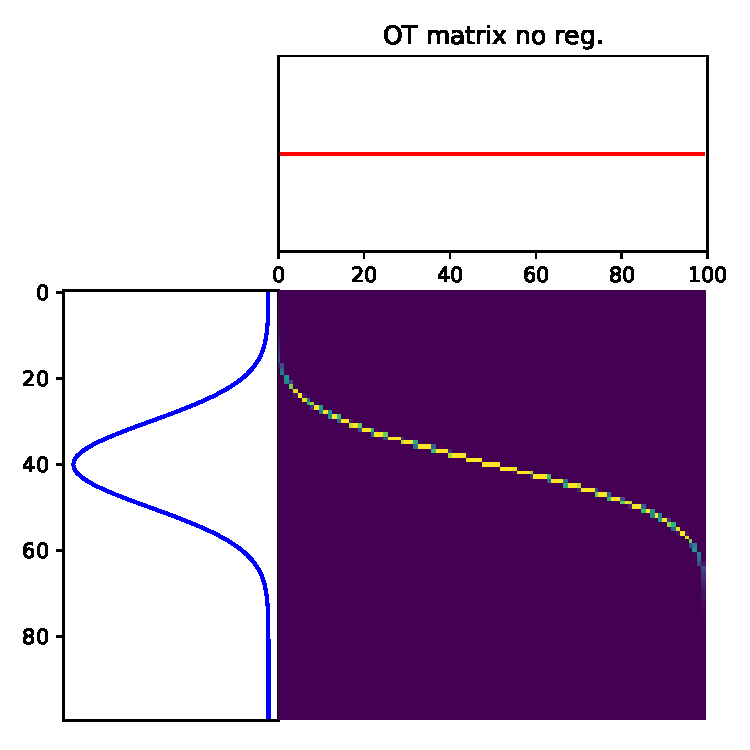
\includegraphics[width=0.32\textwidth]{dist2ToGaussianFig9}\hfill
		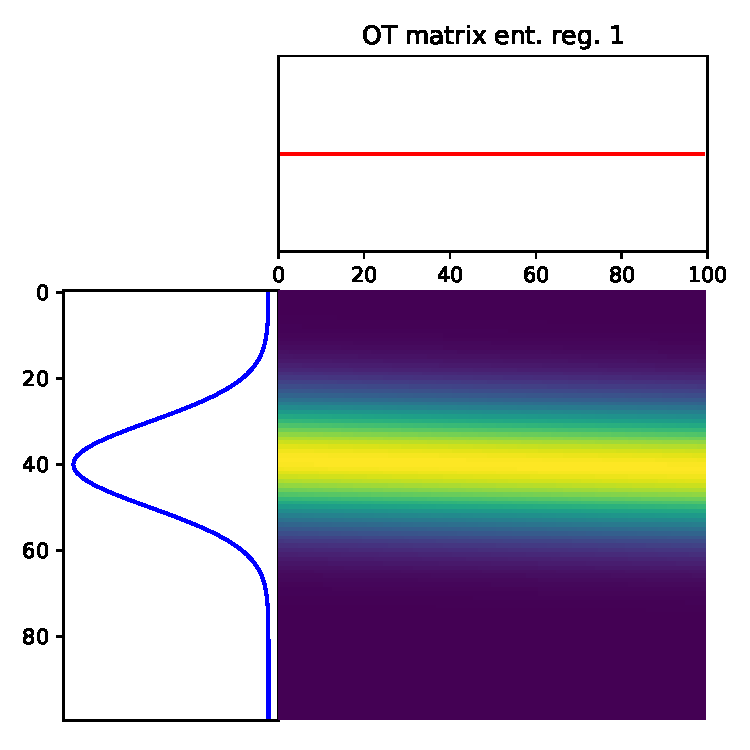
\includegraphics[width=0.32\textwidth]{dist2ToGaussianFig10}\hfill
		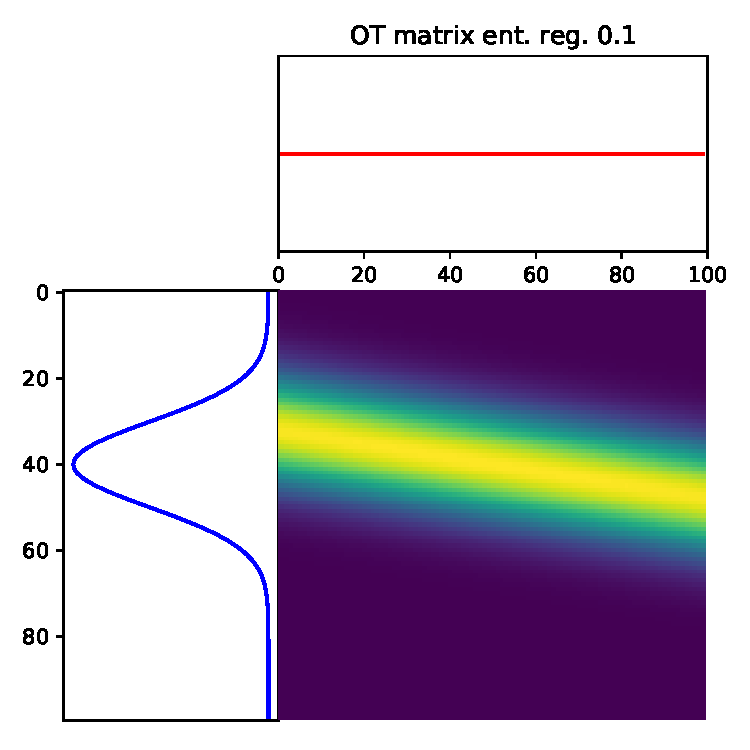
\includegraphics[width=0.32\textwidth]{dist2ToGaussianFig11} \\
		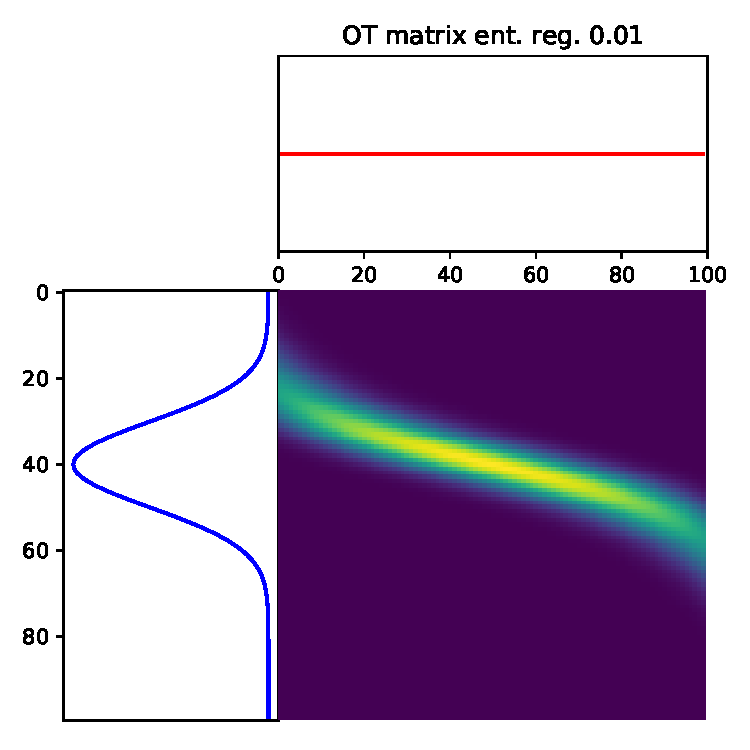
\includegraphics[width=0.32\textwidth]{dist2ToGaussianFig12}\hfill
		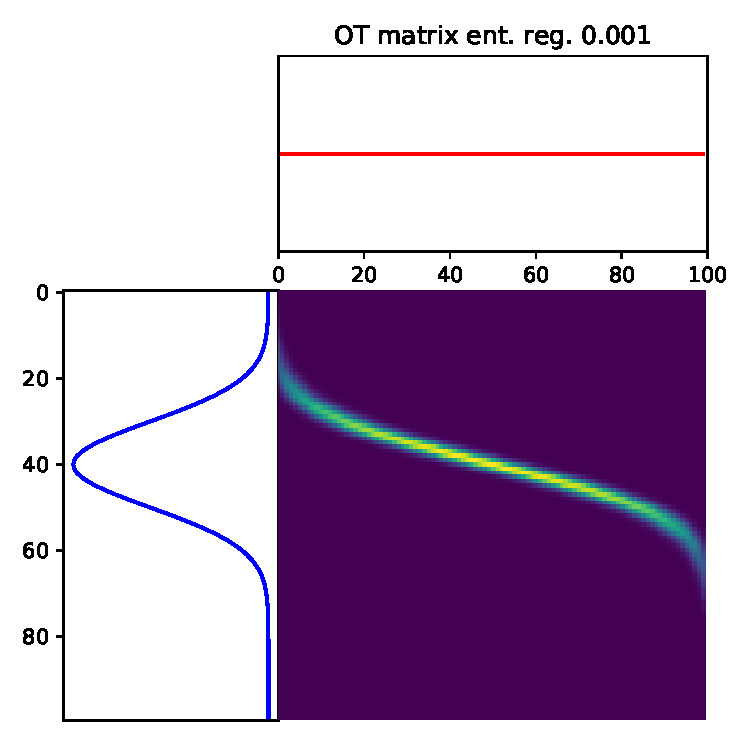
\includegraphics[width=0.32\textwidth]{dist2ToGaussianFig13}\hfill
		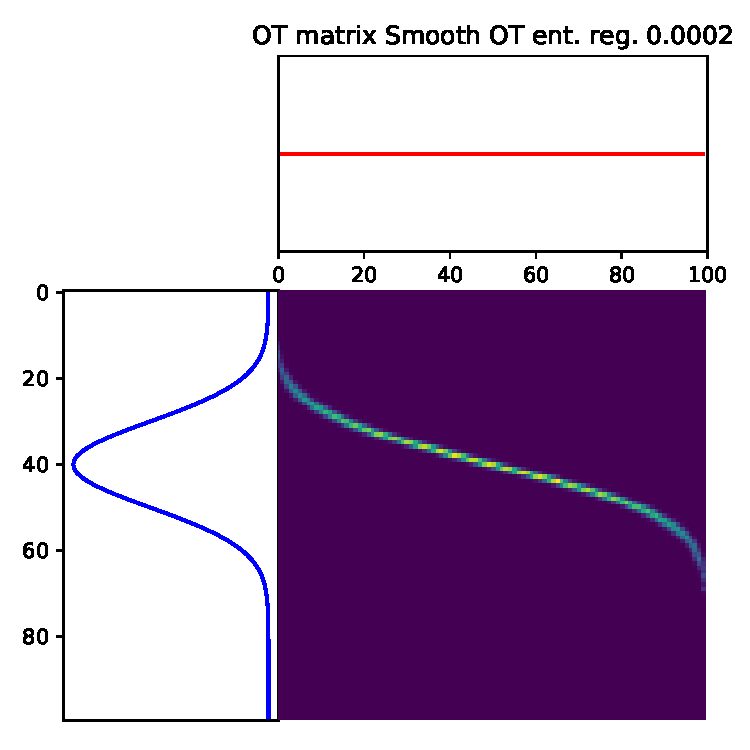
\includegraphics[width=0.32\textwidth]{dist2ToGaussianFig14}\hfill
		\caption{Solutions for unregularized and entropically regularized optimal transport problems, $\varepsilon \in \{ 1, 0.1, 0.	01, 0.001, 0.0001 \}$}\label{RegImages}
	\end{figure}
\end{remark}

With Theorem~\ref{KPAdmitPolishLSC} we already saw that an optimal transport plan exists for (KP). For (RP) however, we require more constraints on our marginal measures. Most importantly, we involve the $L \log L$ spaces from above.

\begin{theorem}[Taken from\ {\cite[Theorem~3.3]{Cla2021}}]\label{RegProbAdmitLLL}
	The problem$\text{\normalfont\ (RP)}$ admits a minimizer $\gamma \in \TP{\mu}{\nu}$ if and only if we have $\mu \in \LLL[\Omega_1]$ and $\nu \in \LLL[\Omega_2]$. In this case, $\gamma \in \LLL$ is unique.
\end{theorem}

\begin{proof}
	Cf.~the proof of\ \cite[Theorem~3.3]{Cla2021}.
\end{proof}

With a solution to (RP), we can achieve weak convergence in the sense of Definition~\ref{WeakConMeas} of the regularized optimal transport plans to a solution of (KP). For this we first consider $X$ and $Y$ as complete metric spaces, and $\Omega_1 \subseteq X, \Omega_2 \subseteq Y, \Omega := \Omega_1 \times \Omega_2$ as compact subsets. Given two probability measures $\mu \in \PM{\Omega_1}$ and $\nu \in \PM{\Omega_2}$, we further require the following two discrete probability measures, weakly converging to $\mu$ and $\nu$ for \Ninf{} respectively, which are defined as
\[ \mu_n := \sum_{i = 1}^n a_i \delta_{x_i}, \nu_n := \sum_{j = 1}^n b_j \delta_{y_j}, \]
with $x_i \in \Omega_1, a_i \ge 0, y_j \in \Omega_2, b_j \ge 0$ for $1 \le i, j \le n$.

With these preliminaries, the following relation between the solutions of (RP) and (KP) can be shown.

\begin{theorem}[Adapted from\ {\cite[Theorem~1]{Seg2018}}]\label{RelatRegSolOrigSolPlan}
	Consider $X$, $Y$, $\Omega_1$, $\Omega_2$, $\Omega$, $\mu$, $\mu_n$, $\nu$ and $\nu_n$ as described above. Let \map[c]{\Omega}{\RZero} be a finite and continuous cost function, and ${(\varepsilon_n)}_{\NinN}$ be a sequence converging to $0$ sufficiently fast with $\varepsilon_n > 0$ for all \NinN. Then for ${(\gamma_n^{\varepsilon_n})}_{\NinN}$, the sequence of solutions of$\text{\normalfont\ (RP)}$ between $\mu_n$ and $\nu_n$ with $\varepsilon = \varepsilon_n$, there exists a subsequence ${(\gamma_{n_k}^{\varepsilon_{n_k}})}_{\NinN[k]}$ that weakly converges to a solution $\gamma$ of$\text{\normalfont\ (KP)}$ between $\mu$ and $\nu$ for \Ninf.
\end{theorem}

\begin{proof}
	This proof was adapted from the proof of\ \cite[Theorem~1]{Seg2018}.

	We consider $\gamma_n$ the solution of (KP) between $\mu_n$ and $\nu_n$ with maximum entropy. According to\ \cite[Theorem~5.20]{Vill2009}, there now exists a subsequence which weakly converges to a solution $\gamma$ of the same problem between $\mu$ and $\nu$. We continue to label this subsequence as $\gamma_n$, and further take the same indices to form a subsequence from the solutions of (RP) between $\mu_n$ and $\nu_n$, labelling it $\gamma_n^{\varepsilon_n}$. The solutions of (RP) exist due to the discrete measures $\mu_n, \nu_n$ reducing the integral over $\Omega_1$ and $\Omega_2$ respectively to a finite sum over their masses $x_i, y_j$, hence allowing for the application of Theorem~\ref{RegProbAdmitLLL}. By expanding the following integral for $g \in \CF[b]{\Omega}$
	\[ \Bigg\lvert \int\limits_{\Omega} g~\D[\gamma_n^{\varepsilon_n}] - \int\limits_{\Omega} g~\D[\gamma] \Bigg\rvert \le \Bigg\lvert \int\limits_{\Omega} g~\D[\gamma_n^{\varepsilon_n}] - \int\limits_{\Omega} g~\D[\gamma_n] \Bigg\rvert + \Bigg\lvert \int\limits_{\Omega} g~\D[\gamma_n] - \int\limits_{\Omega} g~\D[\gamma] \Bigg\rvert, \]
	we have to show that the left summand on the right-hand side converges to $0$, because the other summand converges by the previously mentioned statement of\ \cite{Vill2009}. As $\gamma_n^{\varepsilon_n}$ and $\gamma_n$ are solutions to optimal transport problems between discrete measures, we can replace the integral over $\Omega$ with sums over the masses of both measures and obtain
	\[ \Bigg\lvert \sum\limits_{i, j = 1}^n g(x_i, y_j) \gamma_n^{\varepsilon_n}(x_i, y_j) - \sum\limits_{i, j = 1}^n g(x_i, y_j) \gamma_n(x_i, y_j) \Bigg\rvert \le M_g \Vert \gamma_n^{\varepsilon_n} - \gamma_n \Vert_{1}^{n \times n}, \]
	where $\Vert \gamma_n^{\varepsilon_n} - \gamma_n \Vert_{1}^{n \times n} := \sum\limits_{i, j = 1}^n \big\lvert \gamma_n^{\varepsilon_n}(x_i, y_j) - \gamma_n(x_i, y_j) \big\rvert$ and $M_g := \max g(x_i, y_j)$ over $1 \le i, j \le n$. Adapting a result from\ \cite[specifically Equation~2 in the proof of Proposition~3.1]{Comi1994}, there exist $M_{c_n, \mu_n, \nu_n}, \lambda_{c_n, \mu_n, \nu_n} > 0$ such that
	\[ \Vert \gamma_n^{\varepsilon_n} - \gamma_n \Vert_1^{n \times n} \le M_{c_n, \mu_n, \nu_n} \exp\left( \frac{-\lambda_{c_n, \mu_n, \nu_n}}{\varepsilon_n} \right), \]
	with $c_n := {\big( c(x_i, y_j) \big)}_{i, j = 1}^n$. To show the convergence of the right-hand side, we finally choose $\varepsilon_n = \lambda_{c_n, \mu_n, \nu_n} \cdot {\ln\left( n\,M_{c_n, \mu_n, \nu_n} \right)}^{-1} \rightarrow 0, \Ninf$.
\end{proof}

Before handling the dual problem of (RP), we investigate the \textit{barycentric projection} in the next section. The barycentric projection is a specific method of obtaining a transport map from a transport plan, allowing us to take a solution of (RP), and get a solution of (MP) in return.

The results of the following two sections will then be combined in the last section of this part to enable the estimation of optimal transport plans and maps for large-scale problems.

\section{The Barycentric Projection}\label{BaryProj}

In the first part, specifically in Theorem~\ref{IndPlansDense}, we already saw that the set of transport plans induced by transport maps is densely contained within the set of all transport maps \TP{\mu}{\nu}. We are now interested in finding a transport map from our regularized optimal transport plan, i.e.~a solution to (RP) between $\mu$ and $\nu$, since the handling of a mapping instead of a joint measure is often advantageous in direct applications. We have already seen in Theorem~\ref{InfCoincide}, that when $\mu$ is atomless, such a transport map is directly related to the accompanying transport plan. This suggests that we start with a weakly convergent subsequence of regularized transport plans and apply a transformation which will then result in a sequence weakly converging to an optimal transport map. The transformation chosen by\ \cite{Seg2018}, is the so-called barycentric projection.

\begin{definition}[Barycentric Projection; adapted from\ {\cite[Definition~1]{Seg2018}}]\label{BarCentrProj}
	We consider a transport plan $\gamma \in \TP{\mu}{\nu}$ and a convex cost function $\map[d]{\Omega_2 \times \Omega_2}{\RZero \cup \{ \infty \}}$. Then the \textbf{barycentric projection} of $\gamma$ at $x \in \Omega_1$ is defined as
	\[ \bar{\gamma}(x) := \argmin\limits_{z \in \Omega_2} \int\limits_{\Omega_2} d(z, y)~\Dx[x, y]{\gamma}. \]
	If $d(x, y) = \Vert x - y \Vert_2^2$, where $\Vert \cdot \Vert_2$ is the Euclidean norm, the barycentric projection has the closed form
	\[ \bar{\gamma}(x) = \int\limits_{\Omega_2} y~\Dx[x, y]{\gamma}. \]
	If $c(x, y) = \Vert x - y \Vert_2^2$, according to\ \cite{Seg2018}, it can be further shown that the barycentric projection of an optimal transport plan for (KP) is already an optimal transport map for (MP).
\end{definition}

Similarly to Theorem~\ref{RelatRegSolOrigSolPlan}, we will be considering $X = Y = \R^d$, with $\Omega_1, \Omega_2 \subseteq \R^d, \Omega := \Omega_1 \times \Omega_2$ compact, a continuous measure $\mu \in \PM{\Omega_1}$ that satisfies\ \cite[Corollary~9.3]{Vill2009}, an arbitrary measure $\nu \in \PM{\Omega_2}$, a continuous cost function $\map[c]{\R^d \times \R^d}{\RZero \cup \{ \infty \}}$, as well as the discrete measures
\[ \mu_n := \frac{1}{n} \sum\limits_{i = 1}^n a_i \delta_{x_i}, \nu_n := \frac{1}{n} \sum\limits_{j = 1}^n b_j \delta_{y_j}, \]
with $x_i \in \Omega_1, a_i \ge 0, y_j \in \Omega_2, b_j \ge 0$ for $1 \le i, j \le n$, weakly converging to $\mu$ and $\nu$ respectively. This then allows us to show the following result, applying the barycentric projection on regularized optimal transport plans to obtain an optimal transport map for (MP).

\begin{theorem}[Adapted from\ {\cite[Theorem~2]{Seg2018}}]\label{RelatRegSolOrigSolMap}
	Consider $X$, $Y$, $\Omega_1$, $\Omega_2$, $\Omega$, $\mu$, $\nu$, $c$, $\mu_n$, $\nu_n$ as described above. Assume that the solutions $\gamma_n$ to$\text{\normalfont\ (KP)}$ between $\mu_n$ and $\nu_n$ are unique for all \NinN. Further let ${(\varepsilon_n)}_{\NinN}$ be a sequence converging sufficiently fast to $0$ with $\varepsilon_n > 0$ for all \NinN, and $d$ be a convex cost function on $\Omega_2 \times \Omega_2$. Then there exists a subsequence ${\big(\bar{\gamma}^{\varepsilon_{n_k}}_{n_k}\big)}_{\NinN[k]}$ such that \weak{\push[\big(id_{\Omega_1}, \bar{\gamma}^{\varepsilon_{n_k}}_{n_k}\big)]{\mu_n}}{\push[(id_{\Omega_1}, T)]{\mu}} for \Ninf, where $T$ is the map solving$\text{\normalfont\ (MP)}$ between $\mu$ and $\nu$, $id_{\Omega_1}$ is the identity map on $\Omega_1$, and $\bar{\gamma}^{\varepsilon_{n_k}}_{n_k}$ is the barycentric projection with respect to the cost function $d$ of the solution $\gamma^{\varepsilon_{n_k}}_{n_k}$ of$\text{\normalfont\ (RP)}$.
\end{theorem}

\begin{proof}
	This proof was adapted from the proof of\ \cite[Theorem~2]{Seg2018}.

	We know that $\push[\bar{\gamma}_n^{\varepsilon_n}]{\mu_n} - \push{\mu} = \push[\bar{\gamma}_n^{\varepsilon_n}]{\mu_n} - \push[\bar{\gamma}_n]{\mu_n} + \push[\bar{\gamma}_n]{\mu_n} - \push{\mu}$. When considering the absolute value of the left-hand side and applying the triangle inequality to the right-hand side, we can prove the weak convergence of our sequence (cf.\ Definition~\ref{WeakConMeas}) claimed in the theorem by proving it for both summands on the right-hand side.	By\ \cite[Corollary~9.3]{Vill2009}, there exists a Monge map between $\mu$ and $\nu$ due to $\mu$ being uniformly continuous on $\Omega_1$ and thus absolutely continuous with respect to the Lebesgue measure. When following the proof of\ \cite[Theorem~2]{Seg2018}, we see that the summand involving $\push[\bar{\gamma}_n]{\mu_n} - \push[T]{\mu}$ converges.
	
	We thus only have to show that for any Lipschitz continuous function $g$ over $\Omega$
	\[ \Bigg\lvert \int\limits_{\Omega} g~\D[{\push[(id_{\Omega_1}, \bar{\gamma}_n^{\varepsilon_n})]{\mu_n}}] - \int\limits_{\Omega} g~\D[{\push[(id_{\Omega_1}, \bar{\gamma}_n)]{\mu_n}}] \Bigg\rvert \rightarrow 0 \]
	for \Ninf{} and $\varepsilon_n$ converging to $0$ sufficiently fast, as \weak{\gamma_n}{T} by\ \cite[Theorem~5.20]{Vill2009}. According to\ \cite{Seg2018}, the optimal transport plan $\gamma_n$ is induced by an optimal map $T_n$, i.e.~$\gamma_n = \push[(id_{\Omega_1}, T_n)]{\mu_n}$, which then further implies $\push[(id_{\Omega_1}, \bar{\gamma}_n)]{\mu_n} = \push[(id_{\Omega_1}, T_n)]{\mu_n}$. This allows us to apply the definition of the push forward and rewrite
	\[ \int\limits_{\Omega} g~\D[{\push[(id_{\Omega_1}, \bar{\gamma}_n^{\varepsilon_n})]{\mu_n}}] = \int\limits_{\Omega} g\big( x, \bar{\gamma}_n^{\varepsilon_n}(x) \big)~\Dx{\mu_n} = \frac{1}{n} \sum\limits_{i = 1}^n g\big( x_i, \bar{\gamma}_n^{\varepsilon_n}(x_i) \big), \]
	\[ \int\limits_{\Omega} g~\D[{\push[(id_{\Omega_1}, \bar{\gamma}_n)]{\mu_n}}] = \int\limits_{\Omega} g\big( x, T_n(x) \big)~\Dx{\mu_n} = \frac{1}{n} \sum\limits_{i = 1}^n g\big( x_i, T_n(x_i) \big). \]
	We apply the closed form of the barycentric projection as given by\ \cite{Seg2018} $\bar{\gamma}(x) = \gamma(x) Y_n$, with $Y_n := {(y_1, \dots, y_n)}^T$ and $\gamma(x) := \big( \gamma(x, y_1), \dots, \gamma(x, y_n) \big)$, to obtain
	\[ \Bigg\lvert \int\limits_{\Omega} g\big( x, \bar{\gamma}_n^{\varepsilon_n}(x) \big)~\Dx{\mu_n} - \int\limits_{\Omega} g\big( x, T_n(x) \big)~\Dx{\mu_n} \Bigg\rvert \le \sum\limits_{i = 1}^n K_g \big\vert \bar{\gamma}_n^{\varepsilon_n}(x_i) - \bar{\gamma}_n(x_i) \big\vert \]
	\[ = n~K_g~\Vert \gamma_n^{\varepsilon_n} Y_n - \gamma_n Y_n \Vert_{\R^{n \times d}, 2} \le n~K_g~\Vert Y_n \Vert_{\R^{n \times d}, 2}^{1/2}~\Vert \gamma_n^{\varepsilon_n} - \gamma_n \Vert^{1/2}_{\R^{n \times n}, 2}, \]
	where we use $K_g < \infty$ the Lipschitz constant of $g$, $\Vert A \Vert_{\R^{d \times n}, 2} = \sigma_{\max}(A^T A)$, $\Vert A \Vert_{\R^{n \times n}, 2} = \sigma_{\max}(A^T A)$, $\gamma_n^{\varepsilon_n} = {\big( \gamma_n^{\varepsilon_n}(x_i, y_j) \big)}_{i, j = 1}^n$, $\gamma_n$ in a similar fashion, and Cauchy-Schwarz is used on the last inequality. Using the same result by\ \cite{Comi1994} as in the proof of Theorem~\ref{RelatRegSolOrigSolPlan}, we can now find $M_{c_n, \mu_n, \nu_n} > 0$ and $\lambda_{c_n, \mu_n, \nu_n} > 0$ such that
	\[ \Vert \gamma_n^{\varepsilon_n} - \gamma_n \Vert^{1/2}_{\R^{n \times n}, 2} \le M_{c_n, \mu_n, \nu_n} \exp\left( \frac{-\lambda_{c_n, \mu_n, \nu_n}}{\varepsilon_n} \right). \]
	Choosing $\varepsilon = \lambda_{c_n, \mu_n, \nu_n} \cdot {\ln\left( n^2 \Vert Y \Vert^{1/2}_{\R^{n \times d}, 2} M_{c_n, \mu_n, \nu_n} \right)}^{-1}$ suffices for the right-hand side of the previous equation to converge to $0$ for any Lipschitz continuous $g$ over $\Omega$, showing \weak{\bar{\gamma}_n^{\varepsilon_n}}{T} for \Ninf.
\end{proof}

As an immediate consequence, we can even avoid the notion of transport plans via the push-forward, and directly formulate the barycentric projection as a transport map.

\begin{corollary}[Taken from\ {\cite[Corollary~1]{Seg2018}}]\label{RelatRegOrigCor}
	With exactly the same assumptions as for Theorem~\ref{RelatRegSolOrigSolMap}, there exists a subsequence ${(n_k)}_{\NinN[k]}, \NinN[n_k]$ for all \NinN[k], such that \weak{\push[\bar{\gamma}^{\varepsilon_{n_k}}_{n_k}]{\mu_{n_k}}}{\nu} for \Ninf.
\end{corollary}

\begin{proof}
	This proof was adapted from the proof of\ \cite[Corollary~1]{Seg2018}.

	We consider $h \in \CF[b]{\Omega_2}$ and further define \map[g]{\Omega}{\R} by $g(x, y) := h(y)$ for all $(x, y) \in \Omega$. As $h$ is bounded and continuous, $g$ is as well. With the same notation as in the proof of Theorem~\ref{RelatRegSolOrigSolMap}, we see that
	\[ \Bigg\lvert \int\limits_{\Omega_2} h~\D[{\push[\bar{\gamma}_n^{\varepsilon_n}]{\mu_n}}] - \int\limits_{\Omega_2} h~\D[{\push{\mu}}] \Bigg\rvert = \Bigg\lvert \int\limits_{\Omega} g~\D[{\push[(id_{\Omega_1}, \bar{\gamma}_n^{\varepsilon_n})]{\mu_n}}] - \int\limits_{\Omega} g~\D[{\push[(id_{\Omega_1}, T)]{\mu}}] \Bigg\rvert. \]
	Applying the theorem mentioned above, we see the left-hand side converging to $0$ for a subsequence if $\varepsilon_n$ converges sufficiently fast. Finally, we can make use of $\push{\mu} = \nu$ to prove the corollary.
\end{proof}

Before we are able to establish large-scale mapping estimation for the optimal transport problem, we need to investigate the dual of the regularized problem. This will occur in a similar way, as was done in Section~\ref{KanDual} for the dual of (KP).

\section{Regularized Duality}\label{RegDual}

As we have previously seen, the regularization term is finite if and only if $\gamma \in \LLL$. By considering (RP) over \LLL{} instead of \TP{\mu}{\nu}, we can also derive a dual problem over $\Lexp[\Omega_1] \times \Lexp[\Omega_2]$. Following the argument put forth in\ \cite[Section~4]{Cla2021}, we define
\[ \Phi(s) := \begin{cases}
	\infty, & s < 0 \\
	s, & 0 \le s \le 1 \\
	\exp(s - 1), & s > 1
\end{cases}, \Psi(s) := \begin{cases}
	- \infty, & s \le 0 \\
	\log(s), & 0 < s \le 1 \\
	s - 1, & s > 1
\end{cases}, \]
\[ u_1 := \begin{cases}
	\exp \left( \frac{\varphi}{\varepsilon} \right), & \varphi \le 0 \\
	\frac{\varphi}{\varepsilon} + 1, & \varphi > 0
\end{cases} \text{, and } u_2 := \begin{cases}
	\exp \left( \frac{\psi}{\varepsilon} \right), & \psi \le 0 \\
	\frac{\psi}{\varepsilon}, & \psi > 0
\end{cases} \]
and obtain $\varphi = \varepsilon \log \big( \Phi(u_1) \big) = \varepsilon \Psi(u_1) \text{ and } \psi = \varepsilon \log \big( \Phi(u_2) \big) = \varepsilon \Psi(u_2)$. When put back into (PD), this gives us
\[ \int\limits_{\Omega_1} \varphi(x)~\Dx{\mu} + \int\limits_{\Omega_2} \psi(y)~\Dx[y]{\nu} - \varepsilon \int\limits_{\Omega} \exp \left( \frac{\varphi(x) + \psi(y) - c(x, y)}{\varepsilon} \right)~\Dx[x, y]{} \]
\[ = \varepsilon \int\limits_{\Omega_1} \Psi\big( u_1(x) \big)~\Dx{\mu} + \varepsilon \int\limits_{\Omega_2} \Psi\big( u_2(y) \big)~\Dx[y]{\nu} - \varepsilon \int\limits F_{\varepsilon}^{\Phi}(x, y)~\Dx[x, y]{}, \]
with $F_{\varepsilon}^{\Phi}(x, y) := \Phi\big( u_1(x) \big) \Phi\big( u_2(y) \big) \exp\left( \frac{-c(x, y)}{\varepsilon} \right)$. We note that $\Phi = \Phi_{\exp}$ on \RZero, suggesting an optimization over ${(u_1, u_2)} \in \Lexp[\Omega_1] \times \Lexp[\Omega_2]$ with $u_1, u_2 \ge 0$ (as the problem would be infeasible for $u_1, u_2 < 0$).

%We are now interested in how this estimate for the regularized problem (RP) may result in a solution for the original problem (KP). Applying Equation~\ref{RegApprTransPlan}, we denote the approximated transport plan for a certain $\varepsilon > 0$ by $\gamma^\varepsilon$.\@~\cite{Seg2018}, Theorem~1, gives us a result regarding the convergence of regularized optimal transport plans.

This argumentation gives rise to the following regularized dual problem.

\begin{definition}[Regularized Dual; adapted from\ {\cite[($\text{D}_{\exp}$)]{Cla2021}}]\label{RegDualProb}
	Let $\mu, \nu, \varepsilon$ as well as $c$ be the same as in Definition~\ref{RegProbs}. We consider the set $\mathcal{F} := \big\{ (f, g) \in \Lexp[\Omega_1] \times \Lexp[\Omega_2] : f, g \ge 0 \big\}$ and define the \textbf{Regularized Dual Problem} as
	\[ \sup\limits_{\mathcal{F}} \left\{ \varepsilon \int\limits_{\Omega_1} \Psi\big( u_1(x) \big)~\Dx{\mu} + \varepsilon \int\limits_{\Omega_2} \Psi\big( u_2(y) \big)~\Dx[y]{\nu} - \varepsilon \int\limits_{\Omega} F_{\varepsilon}^{\Phi}(x, y)~\Dx[x, y]{} \right\}. \]
	This problem will accordingly be labelled as (RD) and its supremum as $\sup \text{(RD)}$. The restriction on $\mathcal{F}$ ensures that all integrals are well-defined.
\end{definition}

Theorem~\ref{RegProbAdmitLLL} gave an existence result for (RP). An analogous statement for (RD) is given by the following theorem, however the class of functions is now $L_{\exp}$ instead of $L \log L$. Following this result, we will investigate the duality between (RP) and (RD), like we investigated the duality between (KP) and (DP) in Section~\ref{KanDual}. Finally, these duality results will provide a way to formulate dual optimality conditions, which will serve as a starting point for plan and mapping estimation for the regularized transport problem.

\begin{theorem}[Adapted from\ {\cite[Theorem~4.6]{Cla2021}}]\label{RegDualAdmit}
	The problem$\text{\normalfont\ (RD)}$ admits a solution $(\bar{u}_1, \bar{u}_2) \in \Lexp[\Omega_1] \times \Lexp[\Omega_2]$.
\end{theorem}

\begin{proof}
	This proof was adapted from the proof of\ \cite[Theorem~4.6]{Cla2021}.
	
	We define the functional
	\[ B(u_1, u_2) := \int\limits_{\Omega} \Phi\big( u_1(x) \big) \Phi\big( u_2(y) \big) \exp\left( \frac{-c(x, y)}{\varepsilon} \right)~\D[(x, y)] \]
	\[ - \int\limits_{\Omega_1} \Psi(u_1)~\D - \int\limits_{\Omega_2} \Psi(u_2)~\D[\nu] \]
	and show that it possesses a minimizer. The value taken by $B$ is finite for e.g.\ $u_1 \equiv u_2 \equiv 1$, allowing us to consider a minimizing sequence ${(u_1^n, u_2^n)}_{\NinN}$ with $(u_1^n, u_2^n) \in \Lexp[\Omega_1] \times \Lexp[\Omega_2]$ for all \NinN. By\ \cite[Lemma~4.2]{Cla2021}, we can assume $\int \Phi_{\exp}(u_1^n)~\D[x] = 1$ without loss of generality. With\ \cite[Lemma~4.4]{Cla2021}, we observe that the norm $\Vert u_2^n \Vert_{\Phi_{\exp}}$ is bounded. By applying the Theorem of Banach-Alaoglu (\ref{Ban-Alao}), we can find a weakly-* convergent subsequence $(u_1^{n_k}, u_2^{n_k})$. Making use of\ \cite[Lemma~4.5]{Cla2021}, the functional $B$ is sequentially weakly-* lower semi-continuous on $\Lexp[\Omega_1] \times \Lexp[\Omega_2]$, showing that the minimum is attained over $\Lexp[\Omega_1] \times \Lexp[\Omega_2]$.
\end{proof}

Continuing the previous argument, we can now substitute $\bar{\phi} = \varepsilon \Psi(\bar{u}_1)$ as well as $\bar{\psi} = \varepsilon \Psi(\bar{u}_2)$ from our dual solutions. We can further assume $\bar{u}_1 > 0$ $\mu$-a.e.\ and $\bar{u}_2 > 0$ $\nu$-a.e., as otherwise $\int \Psi(\bar{u}_1)~\D + \int \Psi(\bar{u}_2)~\D[\nu] = -\infty$, rendering the problem infeasible. The pair $(\bar{\phi}, \bar{\psi})$ however is not guaranteed to be admissible for (PD), i.e.~$\CF[b]{\Omega_1} \times \CF[b]{\Omega_2}$, as even for $\bar{u}_1, \bar{u}_2 > 0$ we do not necessarily get bounds on $\bar{\phi}$ and $\bar{\psi}$, since $\Psi(x) \rightarrow -\infty$ for $x \rightarrow 0$.

If we instead restrict ourselves to the assumptions from Theorem~\ref{RegProbAdmitLLL}, we obtain strong duality between (RP) and (RD).

\begin{theorem}[Adapted from\ {\cite[Proposition~4.7]{Cla2021}}]\label{RegStrongDualityLLL}
	We consider $\mu \in \LLL[\Omega_1], \nu \in \LLL[\Omega_2]$ and $c \in \CF{\Omega}$. Then$\text{\normalfont\ (RP)}$ admits a solution $\bar{\gamma} \in \LLL$,$\text{\normalfont\ (RD)}$ admits a solution $(\bar{u}_1, \bar{u}_2) \in \Lexp[\Omega_1] \times \Lexp[\Omega_2]$, and strong duality holds, i.e.\ $\sup\!\text{\normalfont\,(RD)} = \inf\!\text{\normalfont\,(RP)}$.
\end{theorem}

\begin{proof}
	This proof was taken from the proof\ \cite[Proposition~4.7]{Cla2021}. The existence of a solution follows from Theorem~\ref{RegProbAdmitLLL} and Theorem~\ref{RegDualAdmit}.

	According to\ \cite[Proposition~3.1]{Cla2021}, it suffices to show that strong duality holds between the predual problem and the regularized dual problem, i.e.\ $\sup \text{(PD)} = \sup \text{(RD)}$. For any arbitrary $\alpha \in \CF{\Omega_1}, \beta \in \CF{\Omega_2}$ we set $u_1 := \Psi^{-1}(\alpha/\varepsilon), u_2 := \Psi(\beta/\varepsilon)$ and see that
	\[ \int\limits_{\Omega_1} \alpha~\D + \int\limits_{\Omega_2} \beta~\D[\nu] - \varepsilon \int\limits_\Omega \exp\left( \frac{-c + \alpha + \beta}{\varepsilon} \right)~\D[(x, y)] \le \max\limits_{u_1, u_2 \ge 0} -\varepsilon B(u_1, u_2), \]
	with $B(\cdot, \cdot)$ being defined as in the proof of Theorem~\ref{RegDualAdmit}. By taking the supremum over all $\alpha$ and $\beta$, we get $\sup \text{(PD)} \le \sup \text{(RD)}$.

	To see $\sup \text{(RD)} \le \sup \text{(PD)}$, one may follow the argument put forth by\ \cite{Cla2021} using the theorems of monotone convergence applied to $B$ and dominated convergence applied to a uniformly bounded, weakly-* convergent subsequence.
\end{proof}

As the final result of this section, the following corollary provides two optimality conditions for solutions of (RD), as well as a characterization of primal solutions to (RP) in terms of its optimal dual variables.

\begin{corollary}[Conditions on Dual Optimality; adapted from\ {\cite[Theorem~4.8]{Cla2021}}]\label{RegOptCond}
	Let $\mu \in \LLL[\Omega_1], \nu \in \LLL[\Omega_2]$ and $c \in \CF{\Omega}$, as in Theorem~\ref{RegStrongDualityLLL}. Then, for $\mu$-a.e.\ $x \in \Omega_1$ and $\nu$-a.e.\ $y \in \Omega_2$ all dual solutions $(\bar{u}_1, \bar{u}_2) \in \Lexp[\Omega_1] \times \Lexp[\Omega_2]$ of$\text{\normalfont\ (RD)}$ satisfy
	\begin{equation}\label{OptCond1}
		\mu(x) = \Phi\big( \bar{u}_1(x) \big) \int\limits_{\Omega_2} \Phi\big( \bar{u}_2(y) \big) \exp \left( \frac{- c(x, y)}{\varepsilon} \right)\D[y],
	\end{equation}
	\begin{equation}\label{OptCond2}
		\nu(y) = \Phi\big( \bar{u}_2(y) \big) \int\limits_{\Omega_1} \Phi\big( \bar{u}_1(x) \big) \exp \left( \frac{- c(x, y)}{\varepsilon} \right)\D[x].
	\end{equation}
	Furthermore, a solution $\bar{\gamma} \in \LLL$ of$\text{\normalfont\ (RP)}$ is defined by
	\[ \bar{\gamma}(x, y) = \Phi\big( \bar{u}_1(x) \big) \Phi\big( \bar{u}_2(y) \big) \exp\left( \frac{- c(x, y)}{\varepsilon} \right). \]
\end{corollary}

\begin{proof}
	Cf.~the proof of\ \cite[Theorem~4.8]{Cla2021}.
\end{proof}

The final section of the second part will contain three algorithms used for mapping estimation. The first makes use of the preceding optimality conditions in Corollary~\ref{RegOptCond}, while the second and the third algorithms will improve on the first to be applicable to large-scale problems. In particular, the dual solutions derived in this section will be estimated by the second algorithm, and a barycentric projection from Section~\ref{BaryProj} approximated for these estimates in the third algorithm.

\section{Stochastic Plan and Mapping Estimation}\label{StoPlanAndMapEst}

We can use the optimality conditions from Corollary~\ref{RegOptCond} to derive the \textit{Sinkhorn algorithm}, as\ \cite[Remark~4.9]{Cla2021}, points out. The idea of this algorithm is twofold: apply Equations~\ref{OptCond1} and\ \ref{OptCond2} to iteratively improve dual variables, and then use the last equation to obtain an estimated optimal transport plan.

For a starting value $u_2^0 \in \Lexp[\Omega_2]$ we define
\[ T_1^{n + 1}(x) := \Phi^{-1} \left( \frac{\mu(x)}{\int_{\Omega_2} \Phi\big( u_2^n(y) \big) \exp\left( \frac{-c(x, y)}{\varepsilon} \right)\D[y]} \right), \]
and
\[ T_2^{n + 1}(y) := \Phi^{-1} \left( \frac{\nu(y)}{\int_{\Omega_2} \Phi\big( u_1^{n + 1}(x) \big) \exp\left( \frac{-c(x, y)}{\varepsilon} \right)\D[x]} \right) \]
for all \NinN, $(x, y) \in \Omega$.

The Sinkhorn algorithm expressed in this setting is given by:
\begin{algorithm}\label{SinkhornAlg}
	\caption{Sinkhorn Algorithm; adapted from\ {\cite[Remark~4.9]{Cla2021}}}
	\KwResult{Optimal dual variables $\bar{u}_1, \bar{u}_2$}
	\KwIn{$\mu \in \PM{\Omega_1}, \nu \in \PM{\Omega_2}, (x, y) \in \Omega, \varepsilon > 0$, cost function $c$, starting variable $u_2^0 \in \Lexp[\Omega_2]$}
	$n := 0$\;
	\While{$\text{\normalfont{}not converged}$}{
		$u_1^{n + 1}(x) := T_1^{n + 1}(x)$\;
		$u_2^{n + 1}(x) := T_2^{n + 1}(y)$\;
		$n := n + 1$\;
	}
\end{algorithm}

Stopping after $N - 1, N > 1$, iterations, we get
\[ \gamma_N(x, y) = \Phi\big( u_1^N(x) \big) \Phi\big( u_2^N(y) \big) \exp\left( \frac{- c(x, y)}{\varepsilon} \right) \]
as an approximate value of transport plan for (RP) at a predetermined value $(x, y)$. Substituting once more with $\exp\left( \frac{\varphi_N(x)}{\varepsilon} \right) = \Phi\big( u_1^N(x) \big)$ as well as $\exp\left( \frac{\psi_N(y)}{\varepsilon} \right) = \Phi\big( u_2^N(y) \big)$, we obtain
\begin{equation}\label{RegApprTransPlan}
	\gamma_N(x, y) = \exp\left( \frac{\varphi_N(x) + \psi_N(y) - c(x, y)}{\varepsilon} \right).
\end{equation}

This $\gamma_N$ now functions as the approximation of an optimal transport plan for the regularized problem. To get an optimal transport map, the barycentric projection of $\gamma_N$ is calculated. In combination with Theorem~\ref{RelatRegSolOrigSolPlan} and Theorem~\ref{RelatRegSolOrigSolMap}, it is sensible to use these estimates in applications.

%This formulation will be used from now on, as it simplifies the following formulae, and by the proof of Theorem~\ref{RegStrongDualityLLL} $\sup\limits_{L_{\exp}} \text{(RD)}$ and $\sup\limits_{\mathcal{C}_b} \text{(PD)}$ coincide.

When considering complex problem settings however, the ever-growing dimensions of the underlying data become problematic. As\ \cite[Section~1, Large-scale OT]{Seg2018} points out, the Sinkhorn algorithm is only useful when considering discrete measures over small samples, because of every single iteration requiring an $\mathcal{O}(n^2)$ cost complexity. Therefore, another approach is required when the underlying measures are continuous or the dimensions of the individual samples get too large.

The procedure proposed by\ \cite{Seg2018} improves on this disadvantage: instead of only computing the approximated dual variables at a specified location $(x, y)$, a neural network is trained to model the continuous case for all values from $\Omega$. In the discrete case, a finite vector representing $\varphi_i = \varphi(x_i)$, and $\psi_j = \psi(y_j)$ respectively, is iteratively improved.

Before continuing, we first give a basic overview on \textit{neural networks}. This overview is based on\ \cite[Chapter~6]{Good2016}, and\ \cite[Section~6.2]{Brag2020}. We then go on to estimate optimal transport plans and finish with the approximation of optimal transport maps with the algorithms given by\ \cite{Seg2018}.

\begin{definition}[Neural Network; adapted from\ {\cite[Chapter~6]{Good2016}}, and\ {\cite[Section~6.2]{Brag2020}}]
	A \textbf{neural network} $\mathcal{H}$ of depth $\NinN[N]$ is a collection of tuples $\cup_{n = 1}^{N} (M_n, b_n, h_n)$. These tuples consist of
	\begin{itemize}
		\item (real-valued) matrices $M_n$,
		\item (real-valued) vectors $b_n$, and
		\item (real-valued) non-linear activation functions $h_n$.
	\end{itemize}
	The dimensions of these matrices, vectors and functions are chosen in such a manner, that for fixed $\NinN[d, l]$ the neural network $\mathcal{H}$ can be evaluated for an input vector $x \in \R^d$, and an output vector $y \in \R^l$ be obtained by applying the recursive formula
	\[ x_{n + 1} = h_n\big( M_n x_n + b_n \big),\ n = 1, \dots, N, \]
	where we define $x_1 := x, y := x_{n + 1}$.

	A neural network with multiple layers between the input and output layers is often called a \textbf{deep neural network}.\ \cite[p. 135]{Brag2020} specifically refers to networks with an arbitrarily large number of layers, where each layer is width-bound, i.e.\ the dimension of each $x_n$, upon which an individual layer acts, is smaller than a fixed size.
\end{definition}

\begin{remark}[Taken from\ {\cite[Formulae~6.48--6.52]{Brag2020}}]
	In practice, examples for typical activation functions are
	\begin{itemize}
		\item $h(x) = \max\{ 0 , x \}$ (Rectifier Linear Unit, ReLU),
		\item $h(x) = \mathbbm{1}_{(0, \infty)}(x)$ (Threshold),
		\item $h(x) = \frac{1}{1 + \exp(-x)}$ (Logistic Sigmoid),
		\item $h(x) = \frac{1}{2} + \frac{1}{\pi} \arctan(x)$ (Arctan Sigmoid), and
		\item $h(x) = \frac{1}{2\pi} \int_{-\infty}^x \exp\big(\!-\frac{1}{2} x^2 \big)$ (Gaussian Sigmoid).
	\end{itemize}
\end{remark}

The entries of the matrices $M_n$ and the vectors $b_n$ are considered as \textit{parameters} $\theta$, and the gradient of the neural network can then be computed with regard to these parameters. From here, we can define the notions of $\nabla \mathcal{H}$ and for $f$ a sufficiently differentiable function $\partial_{\mathcal{H}} f$ (or $\partial_\theta f$). 

We need to adapt the previous definition of $F_\varepsilon$ in Definition~\ref{RegProbs} slightly to include the dual variables:
\[ F_\varepsilon\big( \varphi(x), \psi(y) \big) := \exp\left( \frac{\varphi(x) + \psi(y) - c(x, y)}{\varepsilon} \right). \]
This allows us to state the algorithm estimating optimal dual variables.

\begin{algorithm}\label{OTPlanEstAlg}
	\caption{Transport Plan Estimation; adapted from\ {\cite[Algorithm~1]{Seg2018}}}
	\KwResult{Estimates of optimal dual variables $\varphi, \psi$}
	\KwIn{$\mu \in \PM{\Omega_1}, \nu \in \PM{\Omega_2}, \varepsilon > 0$, cost function $c$, batch size $p$, learning rate $\rho$}
	Initialize $\varphi_0, \psi_0$\;
	$n := 0$\;
	\While{$\text{\normalfont{}not converged}$}{
		sample a batch $(x_1, \dots, x_p)$ from $\mu$\;
		sample a batch $(y_1, \dots, y_p)$ from $\nu$\;
		$\varphi_{n + 1} := \varphi_n + \rho \sum\limits_{i, j = 1}^p \Big( \nabla \varphi_n(x_i) - \varepsilon \partial_{\varphi_n} F_\varepsilon\big( \varphi_n(x_i), \psi_n(y_j) \big) \nabla\varphi_n(x_i) \Big)$\;
		$\psi_{n + 1} := \psi_n + \rho \sum\limits_{i, j = 1}^p \Big( \nabla \psi_n(x_i) - \varepsilon \partial_{\psi_n} F_\varepsilon\big( \varphi_n(x_i), \psi_n(y_j) \big) \nabla\psi_n(y_j) \Big)$\;
		$n := n + 1$\;
	}
\end{algorithm}

To be able to recover the estimated optimal transport plan from the dual variables, we apply Equation~\ref{RegApprTransPlan} in analogy to the Sinkhorn algorithm. As mentioned above, the resulting dual variables take the form of vectors, when $\mu$ and $\nu$ are discrete, and are modelled by neural networks in the continuous case.

The most apparent advantage of this approach according to\ \cite[Section~3, Convergence rates and computational cost comparison]{Seg2018}, is that, in the case of $\mu$ and $\nu$ being discrete, the stochastic gradient descent method converges at a rate of $\mathcal{O}\big( n^{-\frac{1}{2}} \big)$, where $n$ is the iteration number, but only requires a cost of $\mathcal{O}(p^2)$ per iteration. In the case of both measures being continuous, the cost per iteration remains $\mathcal{O}(p^2)$, but convergence can only be ensured up to a stationary point.

Lastly, we want to apply the results of Theorem~\ref{RelatRegSolOrigSolMap} and Corollary~\ref{RelatRegOrigCor} to obtain an estimated optimal transport map. The computation of the desired barycentric projection is however unfeasible for a large-scale problem. To deal with this constraint,\ \cite{Seg2018} train a neural network once more, since this allows for the target map to be defined on all of $\Omega_1$. Parameterizing the map $T_\theta$ as a deep neural network with the parameters $\theta$, the following algorithm can be stated.

\begin{algorithm}\label{OTMapEstAlg}
	\caption{Transport Map Estimation; adapted from\ {\cite[Algorithm~2]{Seg2018}}}
	\KwResult{Estimate $T_\theta$ of the barycentric projection $\bar{\gamma}^\varepsilon$}
	\KwIn{$\mu \in \PM{\Omega_1}, \nu \in \PM{\Omega_2}, \varepsilon > 0$, cost function $c$, convex cost function $d$, batch size $p$, learning rate $\rho$}
	Initialize $T_\theta$\;
	Compute estimates of optimal dual variables $\varphi, \psi$ using Algorithm~\ref{OTPlanEstAlg} with $\mu, \nu, \varepsilon, c, p$ and $\rho$\;
	\While{$\text{\normalfont{}not converged}$}{
		sample a batch $(x_1, \dots, x_p)$ from $\mu$\;
		sample a batch $(y_1, \dots, y_p)$ from $\nu$\;
		$\theta := \theta - \rho \sum\limits_{i, j = 1}^p F_\varepsilon\big( \varphi(x_i), \psi(y_j) \big) \nabla_\theta\,d\big( y_j, T_\theta(x_i) \big)$\;
	}
\end{algorithm}

This algorithm can also be used to compute the opposite barycentric projection $g$ with respect to a convex cost function $d$ on $\Omega_1 \times \Omega_1$. The last term in line~6 of Algorithm~\ref{OTMapEstAlg} should then state $d\big( g(y_j), x_i \big)$ instead. This is due to the symmetry of the optimal transport problem, as\ \cite{Seg2018} points out.

This concludes the thesis, having stated two algorithms that produce an estimated optimal transport plan and map for large-scale optimal transport problems.